\begin{frame}{Raspberry Pi Application}
 \centering
 \vspace*{1em}
 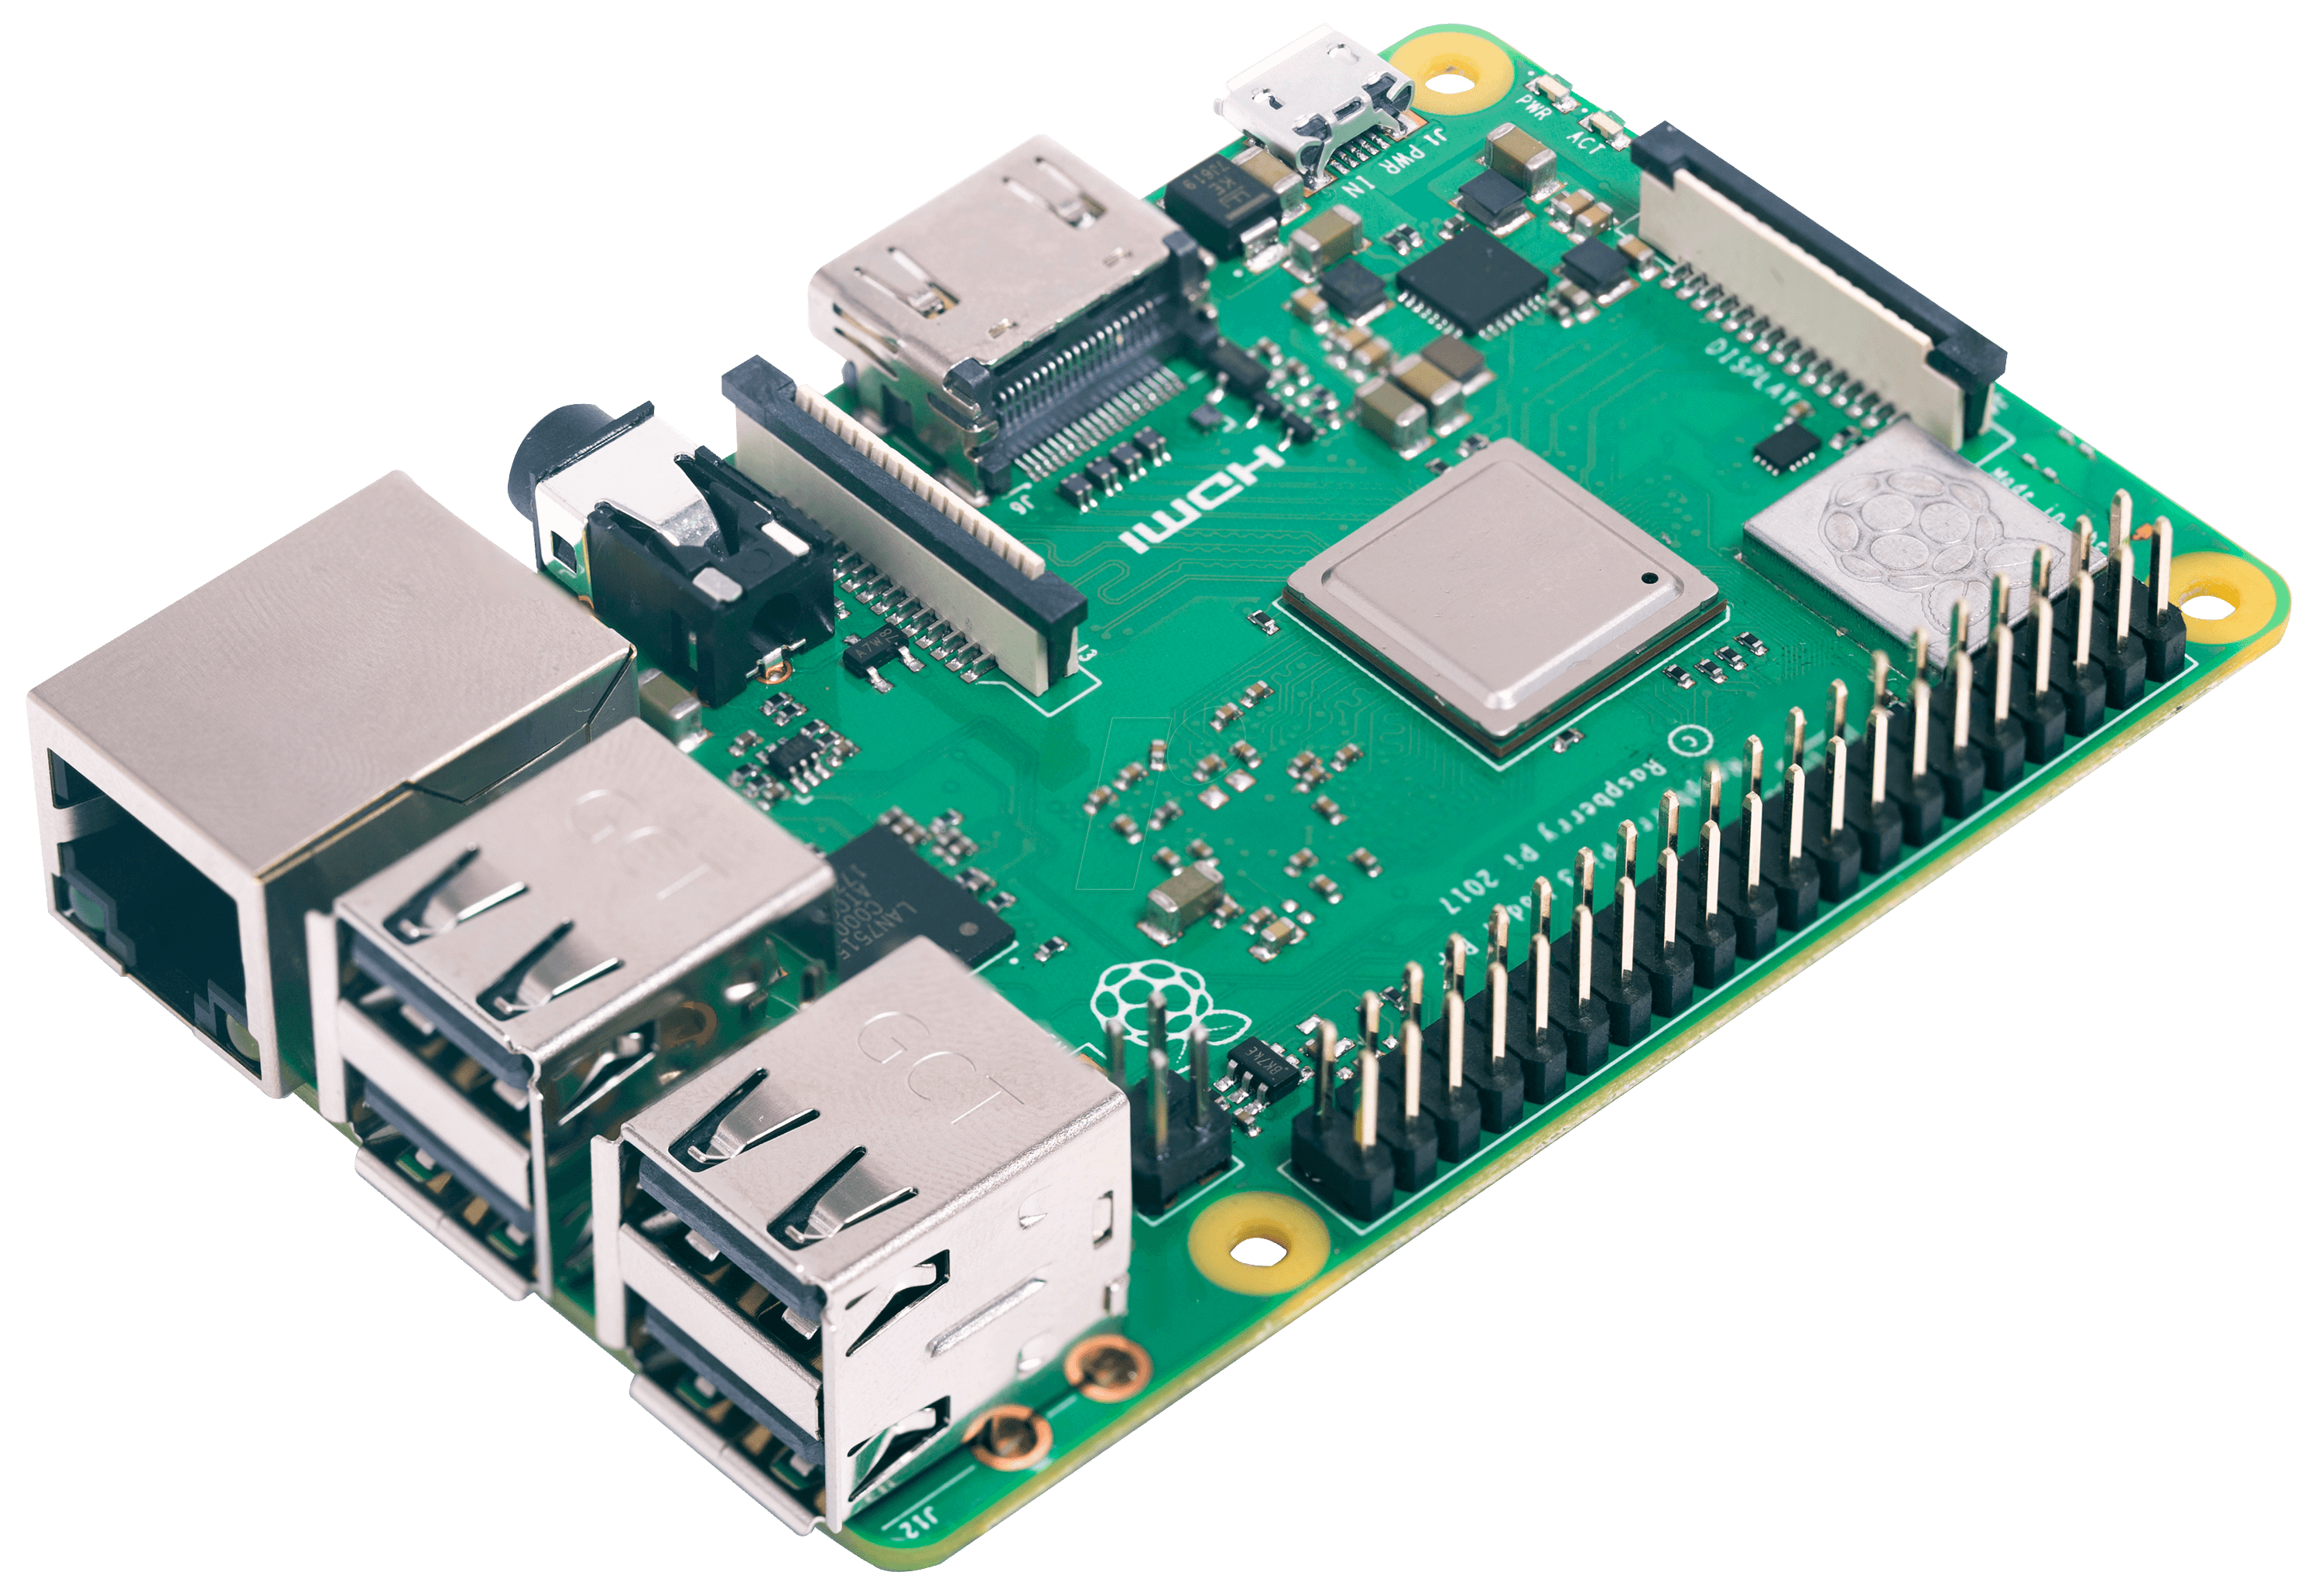
\includegraphics[height=18em]{raspberry-pi-3}
\end{frame}

\begin{frame}{Raspberry Pi Application -- Overview}
  \begin{itemize}
    \item written entirely in Rust
    \item cross-compiled for ARMv7
    \item collects data from 8 sensors
    \item posts sensor data as \textit{JSON} to \textit{Kafka REST}
  \end{itemize}
\end{frame}

\begin{frame}{Raspberry Pi Application -- Rust}
  \begin{itemize}
    \item native code, no interpreter overhead
    \item low latency for sensor measurements
    \item efficient processing of sensor data
    \item built-in package manager and build tool: \texttt{cargo}
  \end{itemize}
\end{frame}

\begin{frame}{Raspberry Pi Application -- Development Workflow}
  \begin{block}{“Hello, world!” program}
    \begin{itemize}
      \item develop on local machine
      \item synchronise code to Raspberry Pi
      \item compile and run directly on Raspberry Pi
    \end{itemize}
  \end{block}
  \begin{block}{\green{Advantages}}
    \begin{itemize}
      \item simple
    \end{itemize}
  \end{block}
  \begin{block}{\red{Disadvantages}}
    \begin{itemize}
      \item synchronisation needed on each change
      \item slow compilation on Raspberry Pi
    \end{itemize}
  \end{block}
\end{frame}

\begin{frame}{Raspberry Pi Application -- Development Workflow}
  \begin{block}{More Sensors, More Dependencies}
    \begin{itemize}
      \item compile time approached 30 minutes for a fresh build
      \item compile time approached 5 minutes for a single iteration
    \end{itemize}
  \end{block}

  \begin{block}{\green{Solution:} Cross Compilation}
    \begin{itemize}
      \item code can be compiled directly on local machine
      \item no need to synchronise on each change
      \item avoids slow compilation on Raspberry Pi
    \end{itemize}
  \end{block}

  \begin{block}{\red{Problem:}}
    \begin{itemize}
      \item most toolchains only available for Linux
    \end{itemize}
  \end{block}
\end{frame}

\begin{frame}{Raspberry Pi Application -- Cross Compilation}
  \begin{block}{Alternatives}
    \begin{itemize}
      \item use Linux virtual machine for cross compilation
      \begin{itemize}
        \item \red{con:} duplicates Rust setup in virtual machine
        \item \red{con:} adds unnecessary complexity
      \end{itemize}
      \item use Docker container for cross compilation
      \begin{itemize}
        \item \red{con:} duplicates Rust setup in container
        \item \red{con:} adds unnecessary complexity
        \item \green{pro:} we are already using Docker in our project
      \end{itemize}
    \end{itemize}
  \end{block}

  \begin{block}{Conclusion}
    \begin{itemize}
      \item Docker preferrable, but still not ideal
    \end{itemize}
  \end{block}
\end{frame}

\begin{frame}{Raspberry Pi Application -- Cross Tool}
  \begin{block}{Features}
    \begin{itemize}
      \item “zero setup cross-compilation”
      \item uses Docker to compile for different targets
      \item wrapper for \texttt{cargo}, Rust's built-in package manager and build system
      \item arbitrary Rust version
    \end{itemize}
  \end{block}

  \begin{block}{\red{Problem}}
    \begin{itemize}
      \item no macOS or Windows support
    \end{itemize}
  \end{block}

  \begin{block}{\green{Solution}}
    \begin{itemize}
      \item implement macOS and Windows support
    \end{itemize}
  \end{block}
\end{frame}

\begin{frame}{Raspberry Pi Application -- How does Cross work?}
  \begin{block}{Workflow}
     \begin{itemize}
       \item if host triple (e.g. \texttt{x86\_64-unknown-linux-gnu}) is supported
         \begin{itemize}
          \item install needed toolchain (e.g. \texttt{armv7-unknown-linux-gnueabi}) using \texttt{rustup}
          \item check if container image for target exists
          \item mount toolchain into container
          \item mount \texttt{cargo} index into container
          \item mount project directory into container
          \item run \texttt{cargo} inside container
         \end{itemize}
       \item otherwise
         \begin{itemize}
           \item fall back to running \texttt{cargo} locally
         \end{itemize}
    \end{itemize}
  \end{block}
\end{frame}

\begin{frame}{Raspberry Pi Application -- Cross: Adding macOS and Windows Support}
  \begin{block}{Fix}
    \begin{itemize}
      \item add macOS and Windows triples to supported host triples
    \end{itemize}
  \end{block}

  \begin{block}{\green{Success}}
    \begin{itemize}
      \item Docker is actually invoked on macOS and on Windows
    \end{itemize}
  \end{block}

  \begin{block}{\red{Problem}}
    \begin{itemize}
      \item compilation on macOS still not working
        \begin{itemize}
          \item \red{Issue:} Docker container (Linux) tries to execute macOS binary
          \item \green{Solution:} override mounted binary directory with empty directory
        \end{itemize}
    \end{itemize}
  \end{block}
\end{frame}

\begin{frame}{Raspberry Pi Application -- Sensors}
  \begin{columns}
    \column{0.5\textwidth}
    \begin{block}{Built-in Sensors}
      \begin{itemize}
        \item memory usage
        \item CPU load
        \item CPU temperature
      \end{itemize}
    \end{block}

    \column{0.5\textwidth}
    \vfill
    \centering
    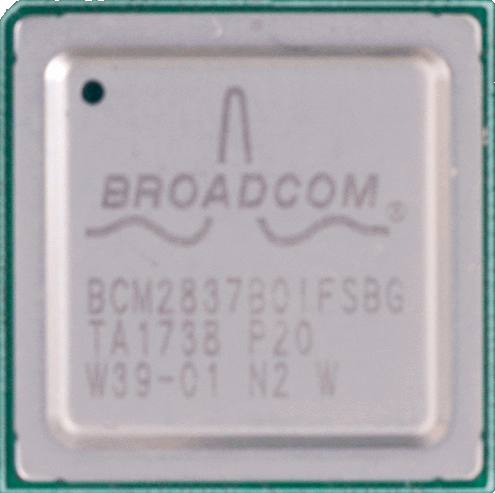
\includegraphics[valign=t,width=5em]{rpi-cpu}
  \end{columns}

  \begin{columns}
    \column{0.5\textwidth}
    \begin{block}{ADS1115 with Photoresistor}
      \begin{itemize}
          \item luminosity
      \end{itemize}
    \end{block}

    \column{0.5\textwidth}
    \vfill
    \centering
    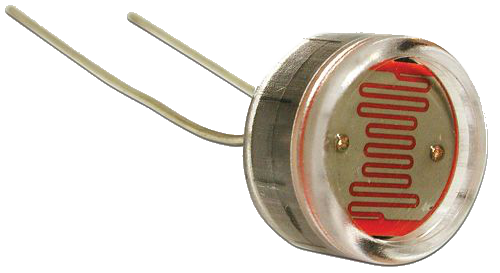
\includegraphics[valign=t,width=5em]{light-sensor}
  \end{columns}
\end{frame}

\begin{frame}{Raspberry Pi Application -- Sensors}
  \begin{columns}
    \column{0.5\textwidth}
    \begin{block}{BMP180}
      \begin{itemize}
        \item air pressure
        \item air temperature
      \end{itemize}
    \end{block}

    \column{0.5\textwidth}
    \vfill
    \centering
    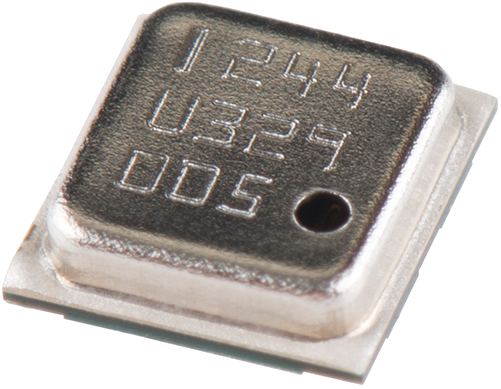
\includegraphics[valign=t,width=5em]{barometric-sensor}
  \end{columns}

  \begin{columns}
    \column{0.5\textwidth}
    \begin{block}{AM2320}
      \begin{itemize}
        \item air humidity
        \item air temperature
      \end{itemize}
    \end{block}

    \column{0.5\textwidth}
    \vfill
    \centering
    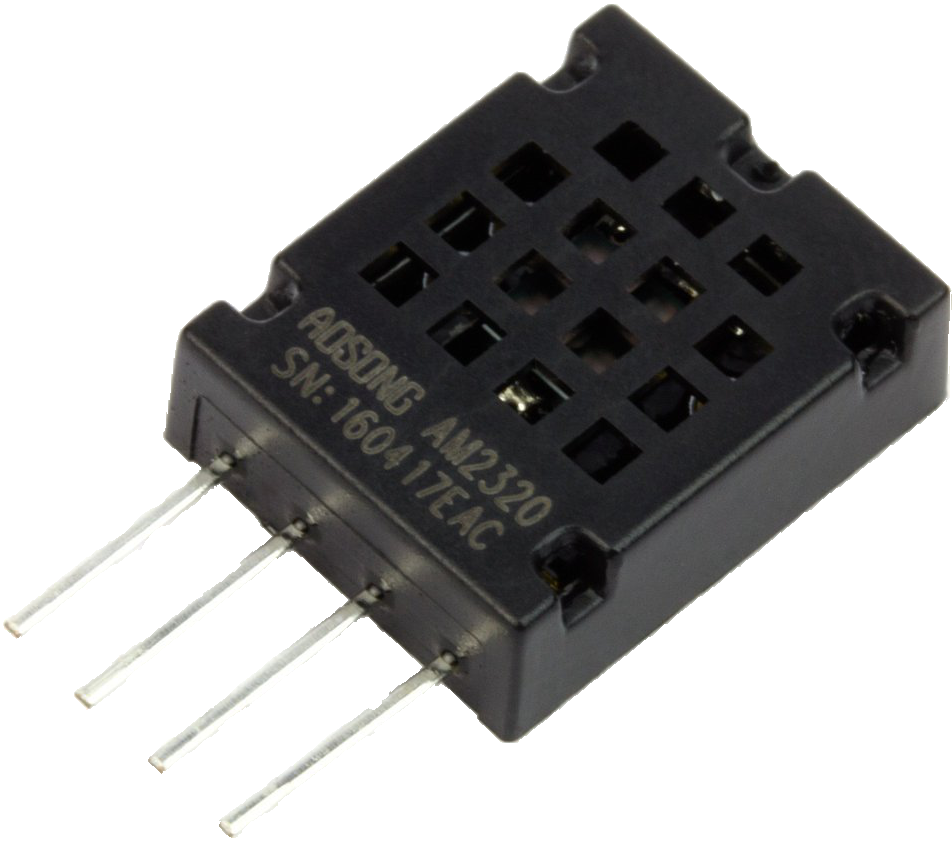
\includegraphics[valign=t,width=5em]{am2320}
  \end{columns}
\end{frame}

\begin{frame}{Raspberry Pi Application -- Sensor Wiring}
  \begin{columns}
    \column{0.35\textwidth}

    \begin{itemize}
      \item {\color{red}red:} 5v power
      \item {\color{orange}orange:} 3.3v power
      \item {\color{black}black:} ground
      \item {\color{purple}purple:} I\textsuperscript{2}C data
      \item {\color{blue}blue:} I\textsuperscript{2}C clock
    \end{itemize}

    \column{0.65\textwidth}
    \vspace*{1em}
    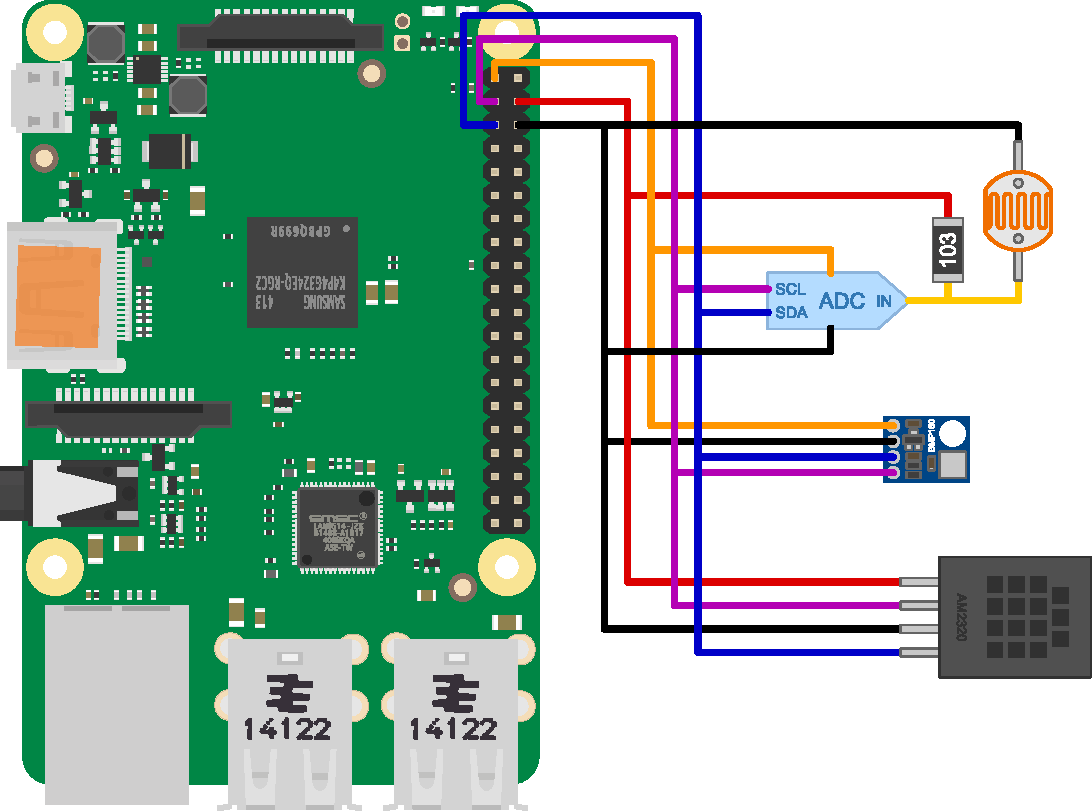
\includegraphics[width=\textwidth]{wiring}
  \end{columns}
\end{frame}

\begin{frame}{Raspberry Pi Application -- Implementation}
  \begin{columns}
    \column{0.5\textwidth}
    \begin{block}{Built-in Sensors}
      \begin{itemize}
        \item \texttt{systemstat} crate
      \end{itemize}
    \end{block}

    \column{0.5\textwidth}
    \vfill
    \centering
    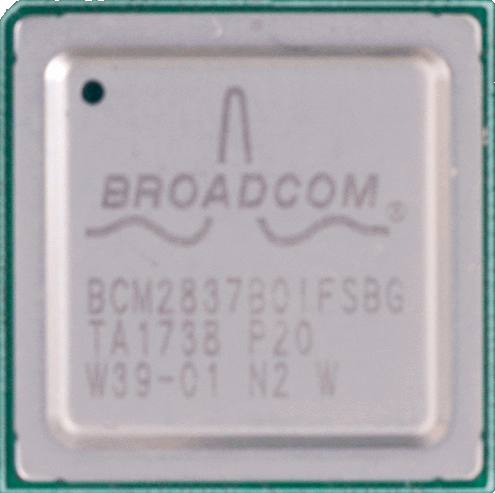
\includegraphics[valign=t,width=5em]{rpi-cpu}
  \end{columns}

  \begin{columns}
    \column{0.5\textwidth}
    \begin{block}{ADS1115 with Photoresistor}
      \begin{itemize}
        \item \texttt{ads1x1x} crate for ADC (analog-to-digital converter)
        \item custom module for approximating luminosity from measured ADC voltage
      \end{itemize}
    \end{block}

    \column{0.5\textwidth}
    \vfill
    \centering
    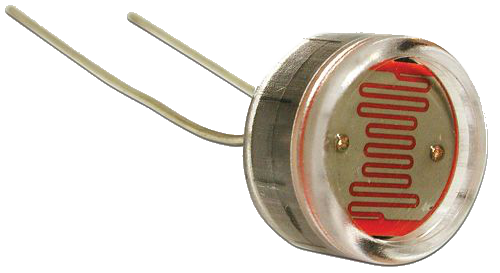
\includegraphics[valign=t,width=5em]{light-sensor}
  \end{columns}
\end{frame}

\begin{frame}{Raspberry Pi Application -- Implementation}
  \begin{columns}
    \column{0.5\textwidth}
    \begin{block}{BMP180}
      \begin{itemize}
        \item \texttt{i2cdev} crate (Linux I2C wrapper)
        \item \texttt{i2cdev\_bmp180} crate (API for BMP180)
        \item \texttt{i2csensors} crate (generalized API for thermometer)
      \end{itemize}
    \end{block}

    \column{0.5\textwidth}
    \vfill
    \centering
    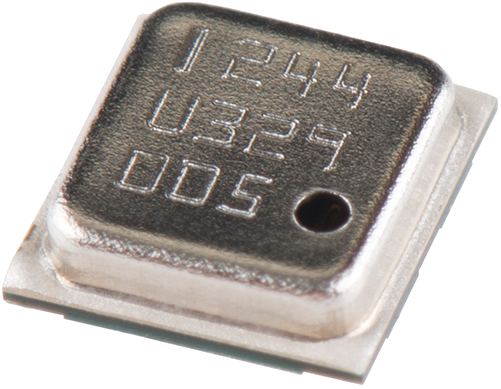
\includegraphics[valign=t,width=5em]{barometric-sensor}
  \end{columns}

  \begin{columns}
    \column{0.5\textwidth}
    \begin{block}{AM2320}
      \begin{itemize}
        \item \texttt{am2320} crate
      \end{itemize}
    \end{block}

    \column{0.5\textwidth}
    \vfill
    \centering
    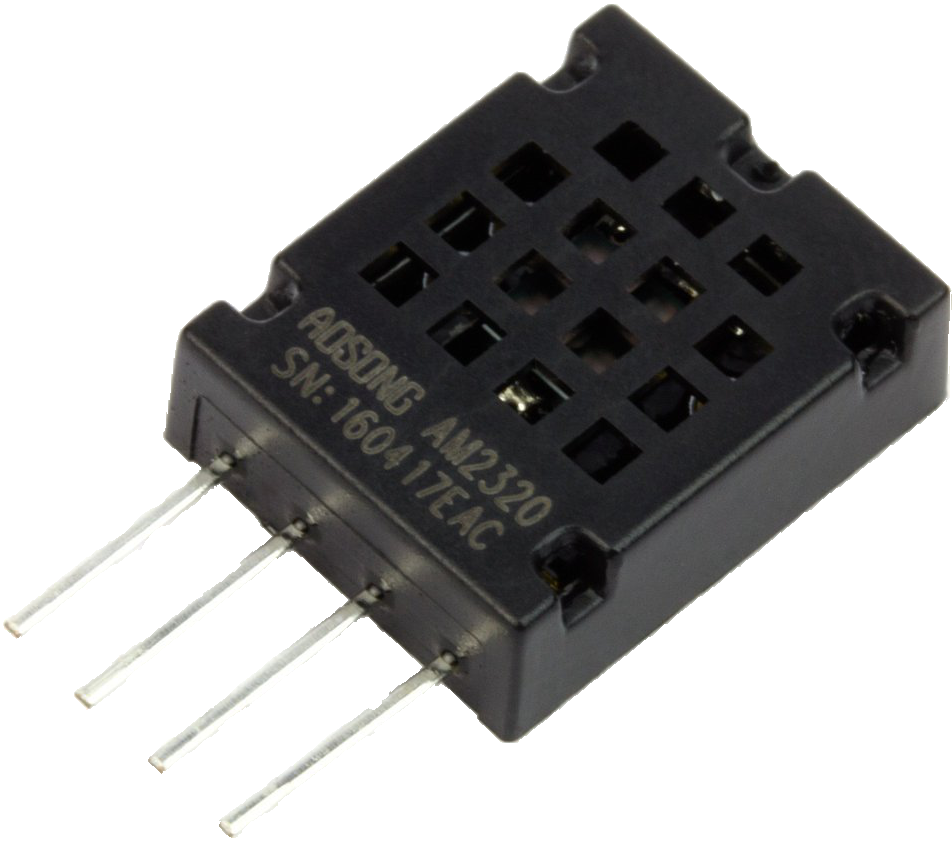
\includegraphics[valign=t,width=5em]{am2320}
  \end{columns}
\end{frame}

\begin{frame}{Raspberry Pi Application -- Implementation}
  \begin{block}{Communication with Serverless Stack}
    \begin{itemize}
      \item \texttt{macaddress} crate
        \begin{itemize}
          \item used for registering the Raspberry Pi in our database (device ID)
        \end{itemize}
      \item \texttt{reqwest} crate
        \begin{itemize}
          \item used for posting requests to Kafka REST endpoint
        \end{itemize}
      \item \texttt{serde} and \texttt{serde\_json} crates
        \begin{itemize}
          \item used for serializing sensor data and building requests
        \end{itemize}
    \end{itemize}
  \end{block}
\end{frame}

\begin{frame}{Raspberry Pi Application -- Implementation}
  \begin{block}{Application Process}
    \begin{enumerate}
      \item post device registration request to Kafka
      \item collect sensor data
      \item send request with collected data to Kafka
      \item sleep 15 seconds
      \item start again at 2.
    \end{enumerate}
  \end{block}
\end{frame}
